\oldpage{405}space of time quiescent. This case would not have excited suspicion,
inasmuch as there seems to be frequently a periodicity in their
actions, but taken in connection with other cases it is a straw which
indicates the quarter from which the wind blows.

Now the question is, does the moon during its various phases exert
various influences which though unperceived by the robust constitution
of perfect health, make themselves felt to the sensitive system
of the invalid, or are these merely striking coincidences? These are
questions of interest to the Physiologist and medical Philosopher,
merely as significant facts, but doubly so to the practitioner to whom
a knowledge of every influence brought to bear upon those under his
charge is essential.

With a hope that others may be induced to make known the result
of their observations, I report these cases.

\begin{figure}[H]
  \centering
  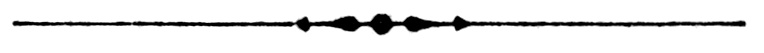
\includegraphics{pages/illustrations/arrow_bullet_divider.jpg}
\end{figure}

\section*{Human Blood a Styptic(?)}

\byline*{\ProperName{O.~Van~Buskirk},\ \md}

\SectionStartWords{I wish} to communicate a few thoughts upon a case which came under
my observation a short time ago, in which I employed human blood as
a styptic with the most gratifying result. To you this may be no new
thing, but to me it is, and it may be to many other junior members of
the profession. From this consideration I thought I would write you
a brief account of the case and the manner in which I employed it.

The case was a lady from whom I extracted a tooth (the first molar),
and it was rather difficult to draw, but it came out whole and without
doing any perceptible damage to the jaw. The hemorrhage was not
very profuse at the time; not more than usual. When she left my office
she seemed as well as usual and continued so for two days, at which
time a profuse hemorrhage took place from the cavity in her jaw. By
means of a decoction of black-oak bark she checked it for about twenty-four
hours when it began again worse than before. I was then sent for
and found her quite weak and sick at her stomach. I applied geranin,
tannic acid, etc., all to no effect. I then took about two ounces of blood,
placed it over the fire and as soon as it came to the boiling point the
solid constituents of the blood coagulated, and left the aqueous portion
clear and limpid. I then poured off the water and left the other over
a slow fire until it assumed a thick, jelly-like form. I took a small lump
of this and filled the cavity and placed over it a small wad of cotton
wadding and directed her to close her jaws so as to keep the remedy in\endinput
